\documentclass[prd,twocolumn,amsmath,amssymb,floatfix,superscriptaddress,nofootinbib]{revtex4-1}
\usepackage{bm}
\usepackage{amsmath}
\usepackage{epsfig}
\usepackage{color}
\usepackage{natbib}
\usepackage{textcase}
\usepackage{graphicx}
\usepackage{ifthen}
\usepackage{xstring}
\usepackage{graphicx}
\usepackage[utf8]{inputenc} 
\usepackage{amssymb}
\usepackage{latexsym}
\usepackage{epstopdf}
\epstopdfsetup{update}
\DeclareGraphicsExtensions{.ps, .png}
\epstopdfDeclareGraphicsRule{.ps}{pdf}{.pdf}{ps2pdf -dEPSCrop -dNOSAFER #1 \OutputFile} 
\usepackage{dcolumn} 
\usepackage{multirow}
\usepackage{appendix}
\usepackage{footnote}
\usepackage{tabularx,ragged2e,booktabs}
\usepackage[normalem]{ulem}
\usepackage{float}
\restylefloat{table}

\newcommand{\Omegamzero}{\Omega_{{\rm m,0}}}
\newcommand{\Rbar}{$\bar{R}$}
\newcommand{\lsc}{\mathcal{L}}
\newcommand{\rhom}{\rho_{\rm m}}
\newcommand{\Mpch}{\mbox{Mpc}/h}
\newcommand{\iMpch}{h/\mbox{Mpc}}
\newcommand{\Msun}{M_\odot}
\newcommand{\Mv}{M_{\rm v}}

\newcommand{\refsec}[1]{section~\ref{sec:#1}}
\newcommand{\refeq}[1]{Eq.~(\ref{eq:#1})}
\newcommand{\refssec}[1]{section~\ref{subsec:#1}}
\newcommand{\reffig}[1]{Fig.~\ref{fig:#1}}
\newcommand{\refFig}[1]{Fig.~\ref{fig:#1}}
\newcommand{\curv}{{\cal R}}
\newcommand{\xef}{x_e^{\rm fid}}
\newcommand{\xmax}{x_e^{\rm max}}
\newcommand{\zmax}{z_{\rm max}}
\newcommand{\zmin}{z_{\rm min}}
\newcommand{\xemin}{x_e^{\rm min}}

\newcommand{\ra}{\rightarrow}
\def\max{_{\mathrm{max}}}
\def\lsim{\mathrel{\raise.3ex\hbox{$$<$$\kern-.75em\lower1ex\hbox{$\sim$}}}}
\def\gsim{\mathrel{\raise.3ex\hbox{$$>$$\kern-.75em\lower1ex\hbox{$\sim$}}}}

\newcommand{\beq}{\begin{equation}}
\newcommand{\eeq}{\end{equation}}

\newcommand{\bea}{\begin{eqnarray}}
\newcommand{\eea}{\end{eqnarray}}

\newcommand{\wh}[1]{\textcolor{blue}{#1}}
\newcommand{\ch}[1]{\textcolor{red}{#1}}

\def\mnras{Mon.\ Not.\ R.\ Astron.\ Soc.\ }
\definecolor{darkgreen}{cmyk}{0.85,0.2,1.00,0.2} 
\definecolor{purple}{cmyk}{0.5,1.0,0,0} 
\def\physrep{Phys.~Rep.}

\definecolor{ultramarine}{rgb}{0.07, 0.04, 0.56}
\definecolor{cadmiumgreen}{rgb}{0.0, 0.42, 0.24}
\definecolor{indigo(dye)}{rgb}{0.0, 0.25, 0.42}
\usepackage[linktocpage=true]{hyperref}
\hypersetup{
colorlinks=true,
citecolor=ultramarine,
linkcolor=cadmiumgreen,
urlcolor=indigo(dye),
pdfauthor={},
pdftitle={},
pdfsubject={}
}


\begin{document}
	
\title{Reionization Planck 2018 ...}

\author{Chen Heinrich}\email{chenhe@caltech.edu}
\affiliation{$Jet\ Propulsion\ Laboratory,\ California\ Institute\ of\ Technology,\ Pasadena,\ California\ 91109,\ USA$}
\affiliation{$California\ Institute\ of\ Technology,\ Pasadena,\ California\ 91109,\ USA$}

\author{Wayne Hu}
\affiliation{Kavli Institute for Cosmological Physics, Enrico Fermi Institute, University of Chicago, Chicago Illinois 60637}
\affiliation{Department of Astronomy \& Astrophysics,
 University of Chicago, Illinois 60637}

\begin{abstract}

...

\end{abstract}
\pacs{}

\maketitle




\section{Introduction}
\label{sec:intro}

\section{Background}

\subsection{Reionization Principal Components}
\subsection{Effective Likelihood from PCs -- Kernel Density Estimate}

\section{Planck 2018 PC Results}
\label{sec:results}

\subsection{Constraints on Principle Components}


\begin{widetext}

\begin{figure}
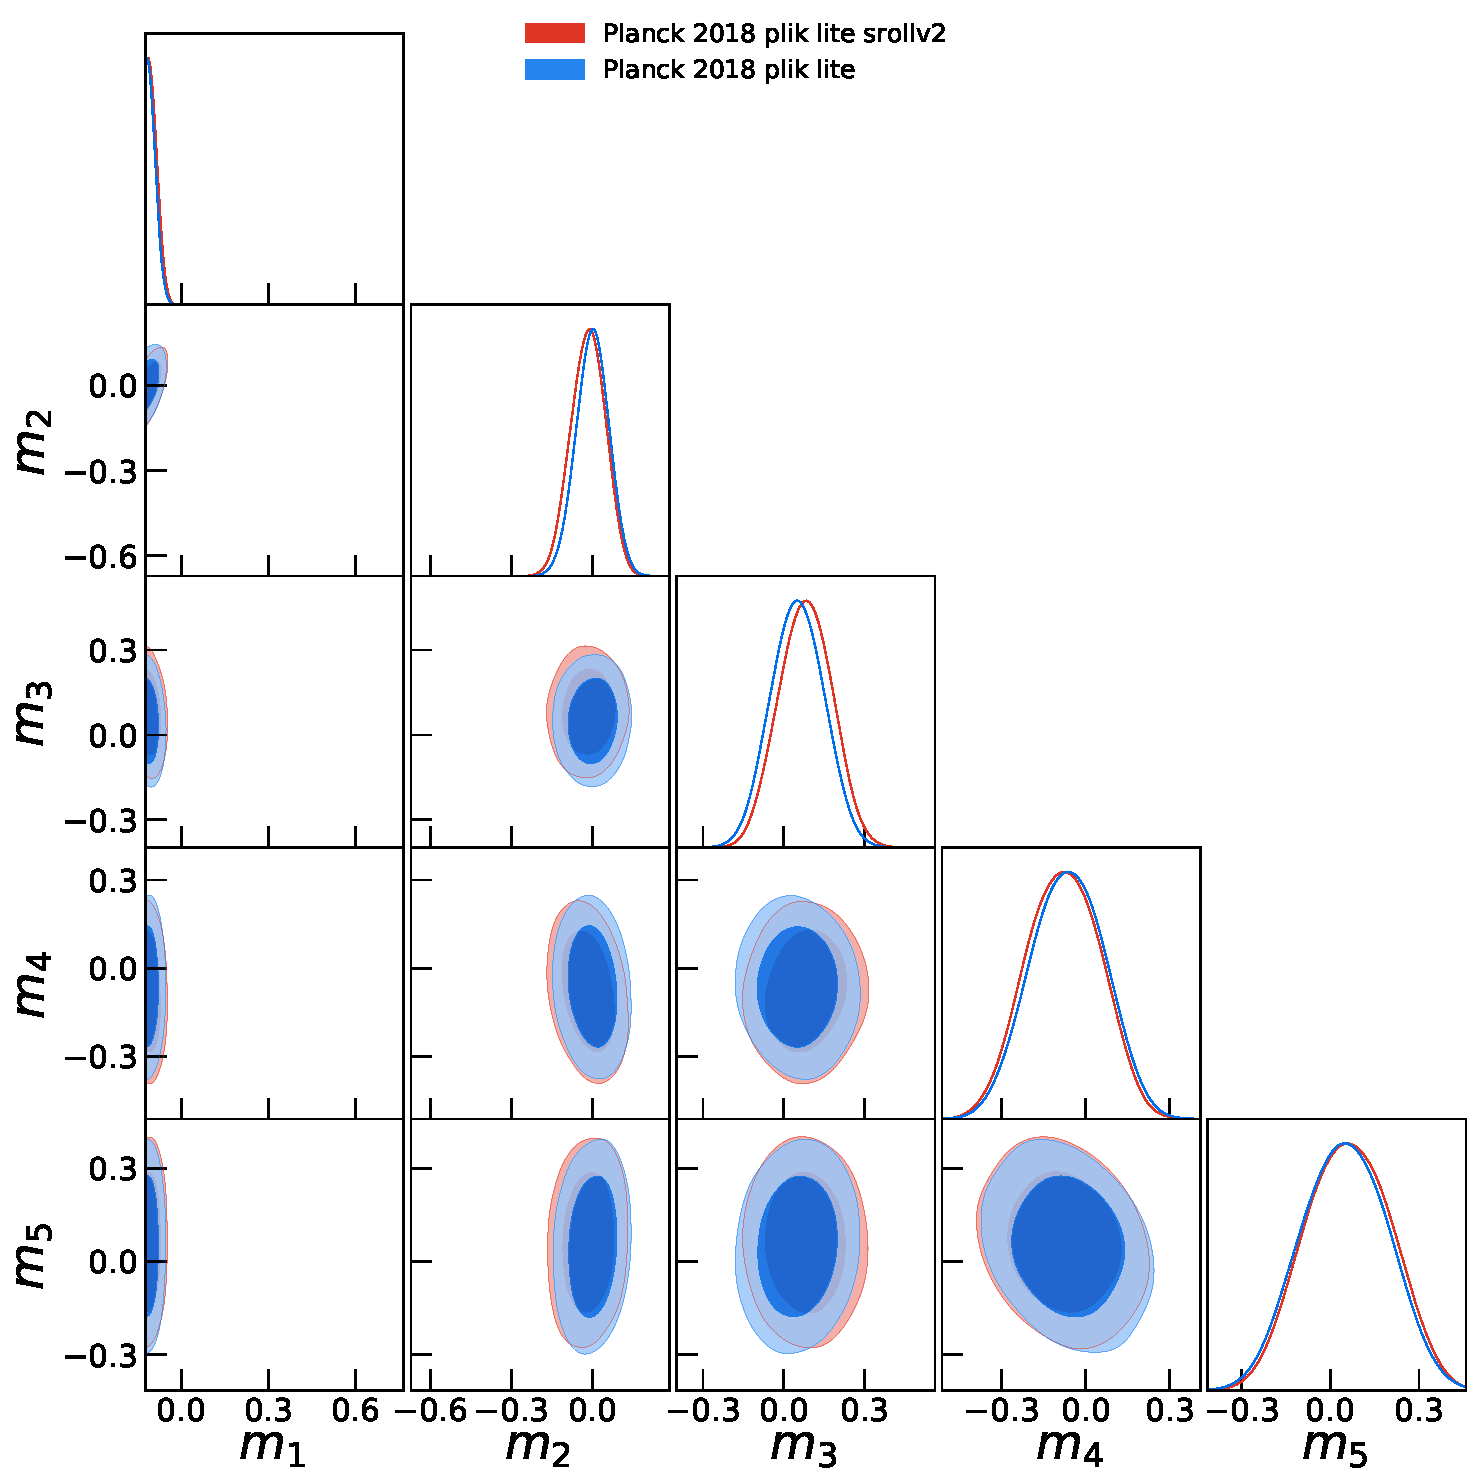
\includegraphics[width=0.7\textwidth]{results/pc_results/plot_mj_triangle_pl18_pc_zmax30_pliklite_srollv2_vs_pl18_pc_zmax30_pliklite.pdf}
\caption{PC chains for zmax = 30 using Planck 2018 srollv2 likelihood vs Planck 2015.
}
\label{fig:plot_mjs}
\end{figure}

\end{widetext}

[Plot: Insert m1-m2 plot about priors]

\begin{figure}
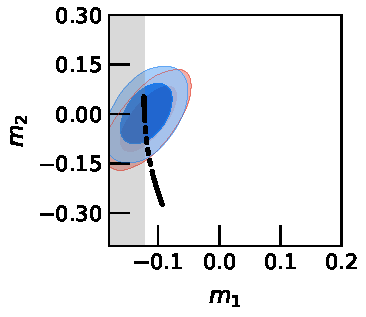
\includegraphics[width=0.4\textwidth]{results/pc_results/plot_m1_m2_pl18_pc_zmax30_pliklite_srollv2_vs_pl18_pc_zmax30_pliklite_wTauTrajectory.pdf}
\caption{m1-m2 plane for zmax = 30 using Planck 2018 srollv2 likelihood vs Planck 2015.
}
\label{fig:plot_m1m2}
\end{figure}



[Plot: Insert m1-m2 plot to show Gaussian covariance does not work]

[Text: recap our appendix from Planck 2015]

[Text: compare with Planck 2015 our PC results]

[Text: statement that zmax = 50 and zmax = 30 are consistent, there is no evidence for high-redshift ionization for $z>30$.]

[Text: make a point that tanh misses high-z again, compare to PCs using the tau($>z$) plot tanh vs PCs.]

[Table: insert table of mean and covariance matrix for the PC components?]


\begin{figure}
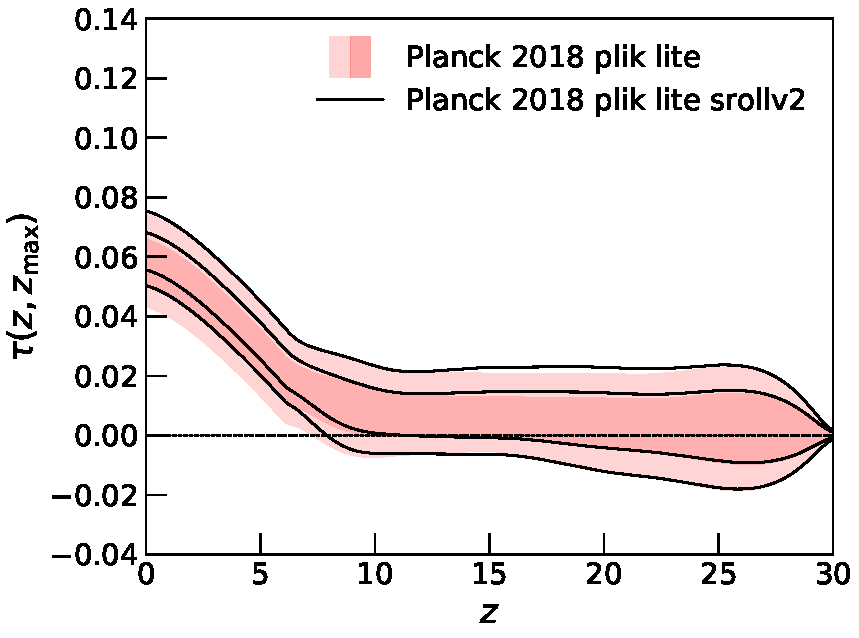
\includegraphics[width=0.48\textwidth]{results/direct_mcmc/pl18_plots_zmax30/plot_pub_tau_gtz_dz_0p1_pl18_pc_zmax30_pliklite_post_0930_and_pl18_pc_zmax30_pliklite_srollv2_0930.pdf}
\caption{PC chains for zmax = 30. Planck 2018 original lowE vs srollv2 likelihood (plik\_lite\_TTTEEE + lowl + simall\_EE vs plik\_lite\_TTTEEE + lowl + sroll2\_EE).
}
\label{fig:}
\end{figure}

\begin{figure}
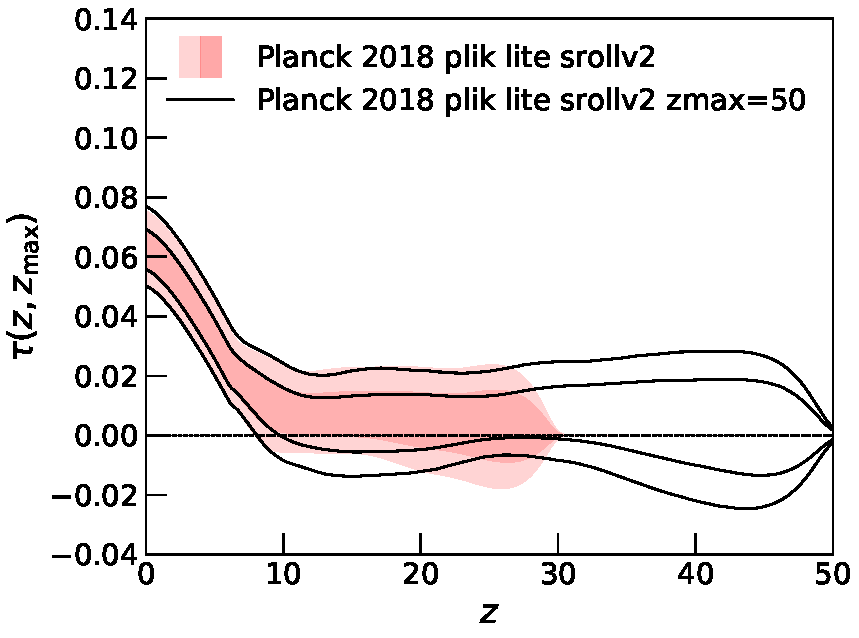
\includegraphics[width=0.48\textwidth]{results/direct_mcmc/pl18_plots_zmax30/plot_pub_tau_gtz_dz_0p1_pl18_pc_zmax30_pliklite_srollv2_0930_and_pl18_pc_zmax50_pliklite_srollv2.pdf}
\caption{Comparing zmax = 30 and 50 PC chains using Planck 2018 original lowE likelihood (plik\_lite\_TTTEEE + lowl + sroll2\_EE). Note that the zmax = 30 uses 5 PCs, whereas the zmax = 50 chains uses 7 PCs. .
}
\label{fig:}
\end{figure}

%Optional
\begin{figure}
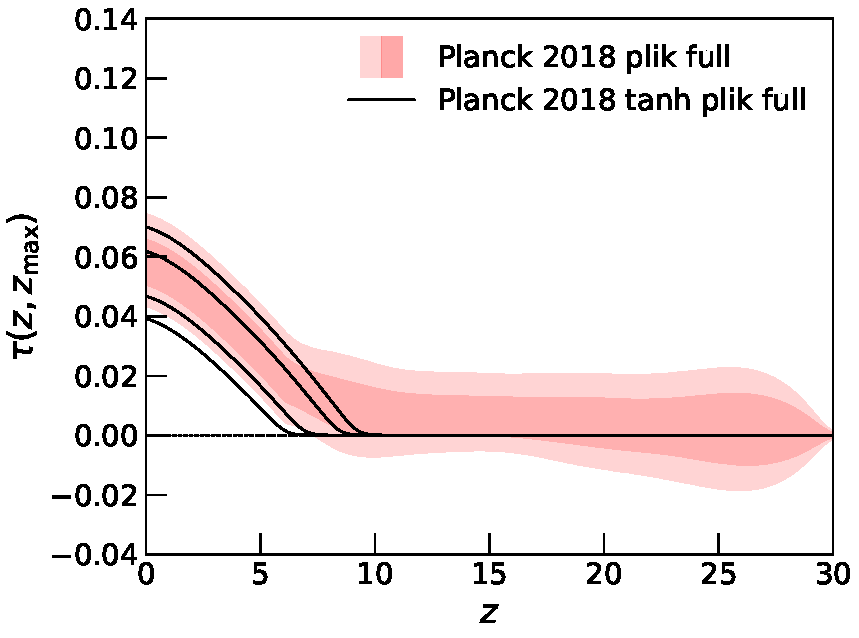
\includegraphics[width=0.5\textwidth]{results/direct_mcmc/pl18_plots_zmax30/plot_pub_tau_gtz_dz_0p1_pl18_pc_zmax30_plikfull_and_pl18_tanh_post_plikfull.pdf}
\caption{PC zmax = 30 vs tanh chains with plik\_full\_TTTEEE for the high-l likelihood.
}
\label{fig:}
\end{figure}


\begin{figure}[t]
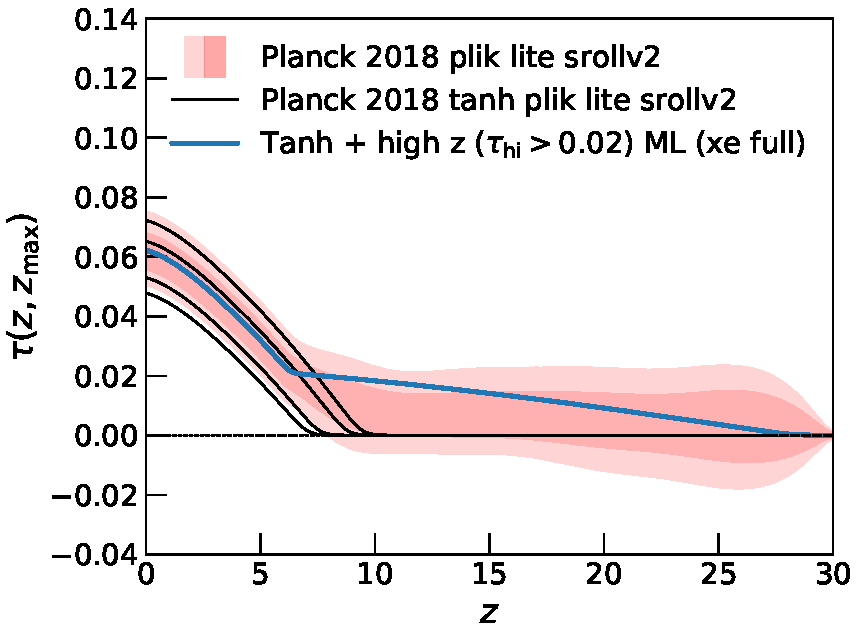
\includegraphics[width=0.40\textwidth]{plots/plot_tau_gtz.pdf}
\caption{...
}
\label{fig:}
\end{figure}


\begin{figure}
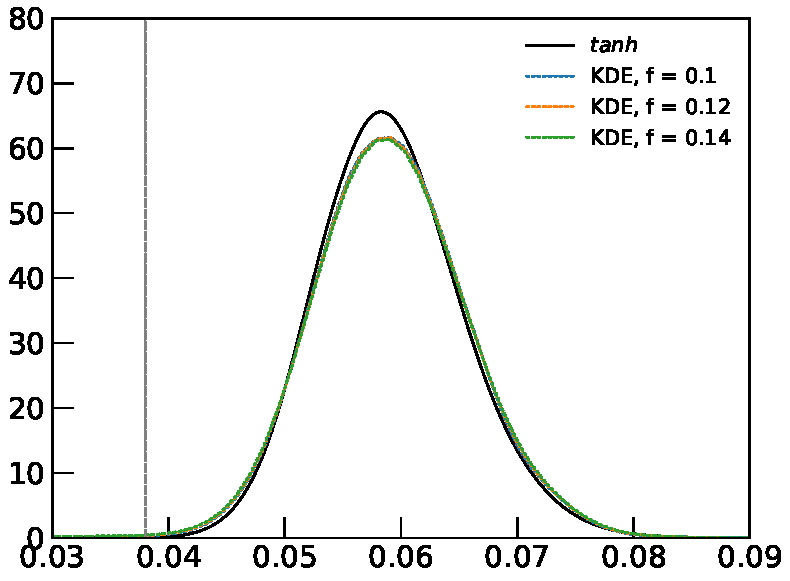
\includegraphics[width=0.40\textwidth]{plots/pl18_pc_zmax30_pliklite_srollv2_1015_tau_posterior_fraccov_1p0_burnin_10000_yes_norm_gaussian0p1_0p12_0p14.pdf}
\caption{...
}
\label{fig:}
\end{figure}


\subsection{A note on priors}

[Text: compare with Planck official results]

[Text: comment that Planck tau(15,30) constraints are too stringent (flex knots). Compare to ours. Point out why.]

[Text: compare with Planck official results, PCs (add comments on priors), FlexKnots]

[*Text (maybe in another section): make a point that dz = 0.5 for tanh may not be sufficient for experiments after Planck. This was for higher tau, so transition happens at higher redshift. Now tau is much lower.]

%%%%%%%%%%%%%%%%%%%%%%%%%%%%%%%%%%%%%%%%%%%%

\section{Effective Likelihood}
\label{sec:effective_likelihood}

\subsection{Code description}
\label{sec:code}

\subsection{Example 1: tanh model}
\label{sec:example1}

\subsection{Example 2: high-z model}
\label{sec:example2}


\begin{figure}
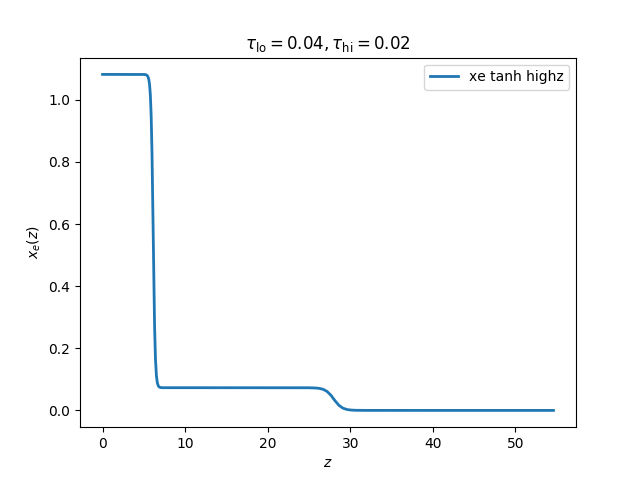
\includegraphics[width=0.5\textwidth]{results/cosmomc_kde/taulo_prior_test/plot_xez_taulo_0p04_tauhi_0p02.png}
\caption{Testing \taulo prior -- Full $x_e(z)$ of the model (\taulo, \tauhi) = (0.04, 0.02) shown in the Fig.~\ref{fig:taulo_prior_test_cl}. 
}
\label{fig:tau_lo_prior_test_xe}
\end{figure}

\begin{figure}
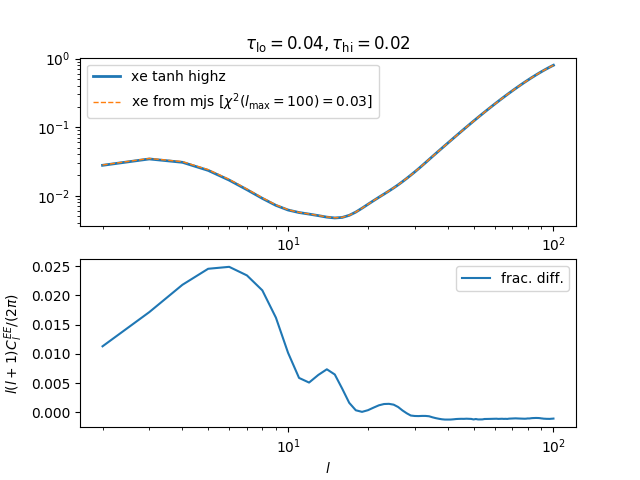
\includegraphics[width=0.5\textwidth]{results/cosmomc_kde/taulo_prior_test/plot_cls_taulo_0p04_tauhi_0p02.png}
\caption{Testing \taulo prior -- testing that \taulo $\geq$ 0.04 as \taulo prior is OK, by calculating $\chi^2$ between $C_l$ from full $x_e(z)$ vs PC decomposition of the model (\taulo, \tauhi) = (0.04, 0.02). 
The $\chi^2 = \sum_{2}^{l_{\rm max}} (\Delta C_l^{EE})^2 / \mathrm{Cov}_l = 0.03$ where $\mathrm{Cov}_l = 2 (C_l^{EE})^2/(2l+1)$. } 
\label{fig:taulo_prior_test_cl}
\end{figure}



\begin{figure}
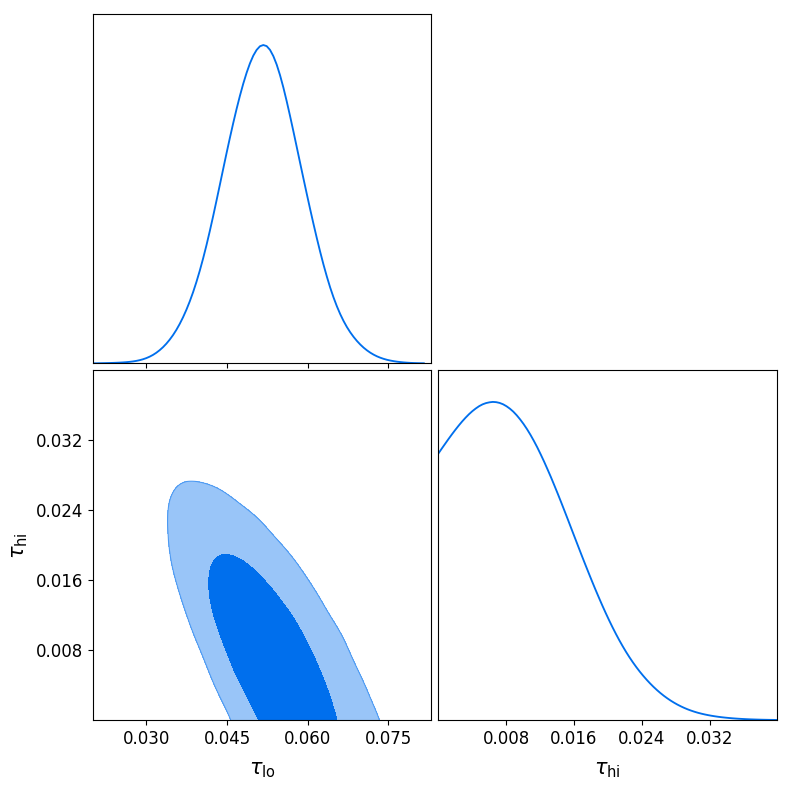
\includegraphics[width=0.5\textwidth]{results/direct_mcmc/two_parameter_model/tauhi_taulo_chains/pl18_tanh_highz_test2_run1_tri.png}
\caption{Direct MCMC chains of the two-parameter model with \tauhi and \taulo: triangle plot of \tauhi and \taulo. The marginalized 1D constraints are \taulo = $0.0516 \pm 0.0076$, \tauhi = $0.0100 \pm   0.0066$. The ML model is \taulo = 0.0543 and \tauhi = 0.0054 corresponding to $z_{\rm re} = 7.68$ and $x_{e, \mathrm{min}} = 0.021$.
}
\label{fig:two_parameter_model_2D_plot}
\end{figure}


\section{Conclusion}
\label{sec:conclusion}


\bibliography{rei.bib}

\appendix

\section{Outline (in progress)}

\begin{enumerate}
	\item{Intro}
	\item{Background}
		\begin{itemize}
			\item{Reionization Principal Components}	
			\item{Kernel Density Estimate}
		\end{itemize}
	\item{Planck 2018 PC results:\\
		- can discuss discrepancy here on high-redshift tau($>$15) constraints.\\
		- compare with our own 2015 PC results
		- zmax = 30 vs 50}
	\item{Effective Likelihood}
		\begin{itemize}
			\item{Code Description}
			\item{Examples - one and two parameter models}
		\end{itemize}
	\item{Discussion}
		
\end{enumerate}


\end{document}
